% ===============================================================
% Document Class ================================================
\documentclass{article}

% ===============================================================
% Graphic Packages ==============================================
\usepackage{graphicx}       % Permite a inclusão de imagens no documento.
\usepackage{tocloft} % Pacote para customização de listas de conteúdos, figuras e tabelas
\usepackage{tikz}           % Ferramenta poderosa para criar gráficos programaticamente dentro do LaTeX.
\usetikzlibrary{calc}       % Extensão da biblioteca TikZ que permite cálculos mais complexos de coordenadas.
\usepackage[portuguese]{babel}
\usepackage{tocloft} % Pacote para customização de listas
\renewcommand{\listfigurename}{Lista de Figuras} % Altera o título para português
\AtBeginDocument{\renewcommand{\contentsname}{Sumário}} % Altera nome de conteudo para sumário
% ===============================================================
% Mathematical Tools ============================================
\usepackage{amsmath}        % Melhora a aparência e a flexibilidade de comandos matemáticos.
\usepackage{siunitx}        % Facilita o uso de unidades do Sistema Internacional e ajuda a formatar números complexos.

% ===============================================================
% Font and Text Appearance ======================================
\usepackage{mathptmx}       % Altera a fonte padrão do documento para Times New Roman.

% ===============================================================
% Table Caption =================================================
\usepackage{booktabs}
\usepackage{caption} 

% ===============================================================
% Table of Contents Customization ===============================
\usepackage{tocloft}  % Oferece controle total sobre a aparência das listas de conteúdos, figuras, tabelas, etc.

% ===============================================================
% Figure Positioning ============================================
\usepackage{float}     % Melhora a interface para definir o posicionamento de objetos flutuantes como figuras e tabelas.

% ===============================================================
% Paragraph Spacing and Indentation =============================
\usepackage{setspace}  % Permite o ajuste fino do espaçamento entre linhas.
\usepackage{indentfirst} % Adiciona indentação ao primeiro parágrafo de cada seção.

% ===============================================================
% Page Layout ===================================================
\usepackage[a4paper, top=3cm, bottom=2cm, left=3cm, right=2cm]{geometry}  % Define as margens de todo o documento.
\setlength{\parindent}{4em}  % Define o tamanho da indentação para todos os parágrafos.
\setlength{\emergencystretch}{3em}

% ===============================================================
% Section Heading Customization =================================
\makeatletter
\renewcommand\paragraph{\@startsection{paragraph}{4}{\z@}%
    {2ex plus 1ex minus .2ex}%
    {1em}%
    {\normalfont\normalsize\bfseries}}
\makeatother

% ===============================================================
% Urls ==========================================================
\usepackage{hyperref} % Para criar links clicáveis
\hypersetup{
    colorlinks=true,
    linkcolor=blue,
    filecolor=magenta,
    urlcolor=blue,
    citecolor=blue,
    pdfborder={0 0 0}  % Remove o quadrado ao redor dos links
}

% ===============================================================
% Bloco de código ===============================================
\usepackage{listings}
\usepackage{xcolor}
\usepackage{courier}
\lstset{
  backgroundcolor=\color[RGB]{249,246,239},
  basicstyle=\ttfamily\footnotesize,
  breaklines=true,
  frame=single,
  numbers=left,
  numberstyle=\tiny\color{gray},
  keywordstyle=\color[RGB]{40,40,255},
  commentstyle=\color[RGB]{0,125,0},
  stringstyle=\color[RGB]{255,0,0},
  showstringspaces=false,
  rulecolor=\color{black},
  captionpos=b,
  abovecaptionskip=5pt,
  belowcaptionskip=5pt,
  xleftmargin=0.15\textwidth,
  xrightmargin=0.15\textwidth,
  morecomment=[l]{//}
}
\renewcommand{\lstlistlistingname}{Lista de Códigos} % Comando para renomear o título da Lista de Códigos

% ===============================================================
% Begin Document ================================================
\begin{document}

% ===============================================================
% Capa ==========================================================
\begin{titlepage}
    \centering
    % Desenhar a margem
    \begin{tikzpicture}[remember picture, overlay]
        \draw[line width = 4pt] ($(current page.north west) + (20mm, -20mm)$) rectangle ($(current page.south east) + (-10mm,10mm)$);
        \draw[line width = 1pt] ($(current page.north west) + (21.5mm,-21.5mm)$) rectangle ($(current page.south east) + (-11.5mm,11.5mm)$);
    \end{tikzpicture}

    % Linha de logos
    
\includegraphics[height=0.151\textwidth]{header/contra-capa/assets/uerj.png}\hfill
    
\includegraphics[height=0.15\textwidth]{header/contra-capa/assets/iprj.jpeg}\hfill

    \vspace{2cm} % Espaço vertical após os logos

    % Informações do curso
    {\Large\bfseries Instituto Politécnico do Estado do Rio de Janeiro \par}
    \vspace{0.5cm}
    {\large Curso de Engenharia da Computação \par}

    \vspace{3cm} % Espaço vertical antes do título da atividade

    % Nome do estudante
    {\large\bfseries Guilherme Cagide Fialho \par}

    \vspace{3cm}

    % Título da atividade
    {\large\bfseries Análise Comparativa de Métodos TVD Aplicados à Solução da Equação de Advecção \par}

    \vfill % Empurra o restante para o fundo da página

    % Local e ano
    {\large\bfseries Nova Friburgo \par}
    \vspace{0.3cm}
    {\large\bfseries 2024 \par}
\end{titlepage}
\newpage % Começa uma nova página após a capa


% ===============================================================
% Contra Capa ===================================================
\begin{titlepage}
    \centering
    % Desenhar a margem
    \begin{tikzpicture}[remember picture, overlay]
        \draw[line width = 4pt] ($(current page.north west) + (20mm, -20mm)$) rectangle ($(current page.south east) + (-10mm,10mm)$);
        \draw[line width = 1pt] ($(current page.north west) + (21.5mm,-21.5mm)$) rectangle ($(current page.south east) + (-11.5mm,11.5mm)$);
    \end{tikzpicture}

    % Linha de logos
    
\includegraphics[height=0.151\textwidth]{header/contra-capa/assets/uerj.png}\hfill
    
\includegraphics[height=0.15\textwidth]{header/contra-capa/assets/iprj.jpeg}\hfill

    \vspace{2cm} % Espaço vertical após os logos

    % Informações do curso
    {\Large\bfseries Instituto Politécnico do Estado do Rio de Janeiro \par}
    \vspace{0.5cm}
    {\large Graduação em Engenharia da Computação \par}

    \vspace{3cm} % Espaço vertical antes do título da atividade

    % Nome do estudante
    {\large Guilherme Cagide Fialho \par}

    \vspace{1.5cm}

    % Título da atividade
    {\large\bfseries Comparativo das solucões das equações de advecção e de advecção-difusão \par}

    \vspace{1cm} % Espaço vertical antes do título da atividade

    % Informações do projeto
    \begin{flushright}
        \begin{minipage}{0.5\textwidth}
            \large
            \raggedleft % Garante que o texto dentro da minipage seja alinhado à direita
            Relatório da Disciplina Métodos Númericos para Equações Diferenciais 2
        \end{minipage}
    \end{flushright}

    \vspace{1.5cm}

    % Informações do orientador
    \begin{flushleft}
        \begin{minipage}{0.5\textwidth}
            \large
            \raggedright
            Orientador: Prof. Hélio Pedro Amaral Souto
        \end{minipage}
    \end{flushleft}


    \vfill % Empurra o restante para o fundo da página

    % Local e ano
    {\large Nova Friburgo \par}
    \vspace{0.3cm}
    {\large 2024 \par}
\end{titlepage}
\newpage % Começa uma nova página após a capa


% ===============================================================
% Resumo ========================================================
\begin{titlepage}
    \thispagestyle{empty} % Remove números de página
    \setstretch{1.5} % Espaçamento entre linhas, certifique-se de que o pacote setspace está incluído em document.tex

    \begin{center}
        \textbf{\Large RESUMO}
    \end{center}


    \vspace{1cm} % Espaço vertical

    \noindent CAGIDE FIALHO, G. Relatório do projeto de Modelagem
    e controle de sistemas. 2024. 54 f. Trabalho de Conclusão de Disciplina Modelagem e Controle de Sistemas (Graduação em
    Engenharia da computação) – Graduação em Engenharia da Computação, Universidade
    do Estado do Rio de Janeiro, Nova Friburgo, 2024.

    \vspace{0.4cm} % Espaço vertical

    Este trabalho explora a modelagem e o controle de um sistema dinâmico do tipo massa-mola-amortecedor, utilizando a plataforma Scilab para desenvolvimento e simulação. O foco do estudo está na implementação de modelos matemáticos para descrever a dinâmica do sistema e na análise de sua resposta sob diversas condições iniciais, sem a aplicação de forças externas. Utilizando a ferramenta Xcos, um componente gráfico do Scilab, realizamos simulações que permitiram uma análise visual e quantitativa das respostas transientes do sistema. O estudo destaca a influência dos parâmetros físicos, como a massa, o coeficiente de amortecimento, e a constante da mola, nas características de resposta do sistema. Além disso, técnicas de controle foram empregadas para ajustar a resposta do sistema, demonstrando como o amortecimento pode contribuir para a estabilização após perturbações e enfatizando a relevância de uma parametrização cuidadosa para alcançar um comportamento eficaz do sistema. Este projeto contribui para a compreensão das teorias de controle aplicáveis em sistemas mecânicos e outros contextos de sistemas dinâmicos na engenharia.
    \vspace{0.4cm} % Espaço vertical

    \textbf{Palavras-chave}: Modelagem e Controle, Sistema Massa-Mola-Amortecedor, Simulação, Scilab, Xcos.
\end{titlepage}


% ===============================================================
% Abstract ======================================================
\begin{titlepage}
    \thispagestyle{empty} % Remove page numbers
    \setstretch{1.5} % Line spacing, make sure the setspace package is included in document.tex

    \begin{center}
        \textbf{\Large ABSTRACT}
    \end{center}

    \vspace{1cm} % Vertical space

    \noindent CAGIDE FIALHO, G. Project Report on Numerical Methods for Differential Equations II. 2024. 25 p. Course Completion Work for Numerical Methods for Differential Equations II (Bachelor’s in Computer Engineering) – Bachelor’s in Computer Engineering, State University of Rio de Janeiro, Nova Friburgo, 2024.

    \vspace{0.4cm} % Vertical space

    This work investigates numerical and analytical solutions to advection and advection-diffusion equations, utilizing Lagrangian methods and Variable Separation. The study focuses on the influence of advection and diffusion coefficients in an infinite domain, exploring how velocity and diffusion coefficient affect the dispersion and transport of solutes. Through detailed numerical simulations, the characteristics of the solutions under various conditions were examined, providing insights into the dynamics of solute in unidimensional flows. Comparative analyses between pure advection and advection-diffusion solutions highlight the significant role of diffusion in modifying the concentration profile, particularly at higher coefficients. This study not only reinforces the theoretical understanding of differential equations in modeling physical phenomena but also serves as a practical reference for engineers and scientists to apply in engineering and environmental contexts.

    \vspace{0.4cm} % Vertical space

    \textbf{Keywords}: Numerical Methods, Advection Equations, Advection-Diffusion, d’Alembert Solution, Variable Separation, Numerical Simulation.
\end{titlepage}


% ===============================================================
% Lista de figuras ==============================================
\section{Desenvolvimento Teórico}

A equação de advecção unidimensional descreve o transporte de uma quantidade conservada, como a concentração de um traçador, ao longo de um eixo espacial. Para resolver essa equação numericamente, é utilizado o método dos Volumes Finitos, que permite a discretização do espaço e do tempo, garantindo uma formulação adequada para a conservação da quantidade transportada \cite{leveque2002finite}. A equação de advecção, em sua forma conservativa, é dada por:

\begin{equation}
    \frac{\partial \Phi}{\partial t} + \frac{\partial}{\partial x} (u \Phi) = 0,
\end{equation}

onde $\Phi$ representa a variável dependente (concentração do traçador) e $u$ é a velocidade de advecção. Com $u$ constante, a equação simplifica-se para:

\begin{equation}
    \frac{\partial \Phi}{\partial t} + u \frac{\partial \Phi}{\partial x} = 0.
\end{equation}

Neste trabalho, a solução numérica é obtida utilizando métodos do tipo \textbf{TVD (Total Variation Diminishing)}. Esses métodos são amplamente reconhecidos por sua capacidade de preservar a monotonicidade da solução e evitar oscilações artificiais, especialmente em regiões com gradientes acentuados ou descontinuidades \cite{harten1983high}. Os métodos implementados são:

\begin{itemize}
    \item \textbf{Limitador de Osher}: Este limitador é projetado para reduzir oscilações artificiais e garantir que a solução permaneça monotônica. Ele é definido como:
          \[
              \phi_{\text{lim}}(\theta) = \max(0, \min(1, \theta)),
          \]
          onde $\theta$ é uma medida da variação local da solução \cite{osher1984rktvd}.

    \item \textbf{Limitador de Sweby}: Este limitador permite maior controle sobre a dissipação, introduzindo um parâmetro ajustável $\beta$. Sua formulação é:
          \[
              \phi_{\text{lim}}(\theta) = \max(0, \min(\beta \theta, \min(1, \theta))),
          \]
          onde valores típicos de $\beta$ estão na faixa $1 \leq \beta \leq 2$ \cite{sweby1984high}.

    \item \textbf{Limitador de Van Albada}: Este limitador equilibra suavidade e precisão, sendo especialmente útil em regiões de gradientes suaves. Sua definição é:
          \[
              \phi_{\text{lim}}(\theta) = \frac{\theta + \theta^2}{1 + \theta^2}.
          \]
          Este limitador é amplamente utilizado devido à sua estabilidade em problemas com gradientes suaves \cite{vanalbada1982family}.
\end{itemize}

Para garantir a estabilidade das simulações, o número de Courant é fixado em $C = 0,8$, respeitando a condição CFL \cite{leveque2002finite}. A condição inicial é definida por uma função composta de uma gaussiana e um valor constante em um intervalo específico, representando um perfil inicial com gradientes suaves e regiões de concentração uniforme. As simulações são realizadas para os instantes de tempo $t = 1$ e $t = 5$, sob condições de contorno periódicas.

Os fluxos nas interfaces dos volumes finitos são calculados considerando os termos anti-difusivos controlados pelos limitadores. A formulação geral do fluxo numérico nos métodos TVD é dada por:
\[
    F_{i+1/2} = u \Phi_i + \frac{u}{2}(1 - C) \phi_{\text{lim}}(\theta_i)(\Phi_{i+1} - \Phi_i),
\]
onde $\theta_i$ é a razão entre os gradientes locais definidos para o intervalo \cite{leveque2002finite}.

Os resultados obtidos serão analisados com gráficos que comparam a solução analítica com as soluções numéricas, permitindo observar a influência de cada limitador na dissipação e dispersão do perfil inicial. Além disso, tabelas apresentarão valores em pontos específicos do domínio para uma análise quantitativa da precisão de cada método.


% ===============================================================
% Lista de tabelas ==============================================
\section{Desenvolvimento Teórico}

A equação de advecção unidimensional descreve o transporte de uma quantidade conservada, como a concentração de um traçador, ao longo de um eixo espacial. Para resolver essa equação numericamente, é utilizado o método dos Volumes Finitos, que permite a discretização do espaço e do tempo, garantindo uma formulação adequada para a conservação da quantidade transportada \cite{leveque2002finite}. A equação de advecção, em sua forma conservativa, é dada por:

\begin{equation}
    \frac{\partial \Phi}{\partial t} + \frac{\partial}{\partial x} (u \Phi) = 0,
\end{equation}

onde $\Phi$ representa a variável dependente (concentração do traçador) e $u$ é a velocidade de advecção. Com $u$ constante, a equação simplifica-se para:

\begin{equation}
    \frac{\partial \Phi}{\partial t} + u \frac{\partial \Phi}{\partial x} = 0.
\end{equation}

Neste trabalho, a solução numérica é obtida utilizando métodos do tipo \textbf{TVD (Total Variation Diminishing)}. Esses métodos são amplamente reconhecidos por sua capacidade de preservar a monotonicidade da solução e evitar oscilações artificiais, especialmente em regiões com gradientes acentuados ou descontinuidades \cite{harten1983high}. Os métodos implementados são:

\begin{itemize}
    \item \textbf{Limitador de Osher}: Este limitador é projetado para reduzir oscilações artificiais e garantir que a solução permaneça monotônica. Ele é definido como:
          \[
              \phi_{\text{lim}}(\theta) = \max(0, \min(1, \theta)),
          \]
          onde $\theta$ é uma medida da variação local da solução \cite{osher1984rktvd}.

    \item \textbf{Limitador de Sweby}: Este limitador permite maior controle sobre a dissipação, introduzindo um parâmetro ajustável $\beta$. Sua formulação é:
          \[
              \phi_{\text{lim}}(\theta) = \max(0, \min(\beta \theta, \min(1, \theta))),
          \]
          onde valores típicos de $\beta$ estão na faixa $1 \leq \beta \leq 2$ \cite{sweby1984high}.

    \item \textbf{Limitador de Van Albada}: Este limitador equilibra suavidade e precisão, sendo especialmente útil em regiões de gradientes suaves. Sua definição é:
          \[
              \phi_{\text{lim}}(\theta) = \frac{\theta + \theta^2}{1 + \theta^2}.
          \]
          Este limitador é amplamente utilizado devido à sua estabilidade em problemas com gradientes suaves \cite{vanalbada1982family}.
\end{itemize}

Para garantir a estabilidade das simulações, o número de Courant é fixado em $C = 0,8$, respeitando a condição CFL \cite{leveque2002finite}. A condição inicial é definida por uma função composta de uma gaussiana e um valor constante em um intervalo específico, representando um perfil inicial com gradientes suaves e regiões de concentração uniforme. As simulações são realizadas para os instantes de tempo $t = 1$ e $t = 5$, sob condições de contorno periódicas.

Os fluxos nas interfaces dos volumes finitos são calculados considerando os termos anti-difusivos controlados pelos limitadores. A formulação geral do fluxo numérico nos métodos TVD é dada por:
\[
    F_{i+1/2} = u \Phi_i + \frac{u}{2}(1 - C) \phi_{\text{lim}}(\theta_i)(\Phi_{i+1} - \Phi_i),
\]
onde $\theta_i$ é a razão entre os gradientes locais definidos para o intervalo \cite{leveque2002finite}.

Os resultados obtidos serão analisados com gráficos que comparam a solução analítica com as soluções numéricas, permitindo observar a influência de cada limitador na dissipação e dispersão do perfil inicial. Além disso, tabelas apresentarão valores em pontos específicos do domínio para uma análise quantitativa da precisão de cada método.


% ===============================================================
% Lista de códigos ==============================================
% \section{Desenvolvimento Teórico}

A equação de advecção unidimensional descreve o transporte de uma quantidade conservada, como a concentração de um traçador, ao longo de um eixo espacial. Para resolver essa equação numericamente, é utilizado o método dos Volumes Finitos, que permite a discretização do espaço e do tempo, garantindo uma formulação adequada para a conservação da quantidade transportada \cite{leveque2002finite}. A equação de advecção, em sua forma conservativa, é dada por:

\begin{equation}
    \frac{\partial \Phi}{\partial t} + \frac{\partial}{\partial x} (u \Phi) = 0,
\end{equation}

onde $\Phi$ representa a variável dependente (concentração do traçador) e $u$ é a velocidade de advecção. Com $u$ constante, a equação simplifica-se para:

\begin{equation}
    \frac{\partial \Phi}{\partial t} + u \frac{\partial \Phi}{\partial x} = 0.
\end{equation}

Neste trabalho, a solução numérica é obtida utilizando métodos do tipo \textbf{TVD (Total Variation Diminishing)}. Esses métodos são amplamente reconhecidos por sua capacidade de preservar a monotonicidade da solução e evitar oscilações artificiais, especialmente em regiões com gradientes acentuados ou descontinuidades \cite{harten1983high}. Os métodos implementados são:

\begin{itemize}
    \item \textbf{Limitador de Osher}: Este limitador é projetado para reduzir oscilações artificiais e garantir que a solução permaneça monotônica. Ele é definido como:
          \[
              \phi_{\text{lim}}(\theta) = \max(0, \min(1, \theta)),
          \]
          onde $\theta$ é uma medida da variação local da solução \cite{osher1984rktvd}.

    \item \textbf{Limitador de Sweby}: Este limitador permite maior controle sobre a dissipação, introduzindo um parâmetro ajustável $\beta$. Sua formulação é:
          \[
              \phi_{\text{lim}}(\theta) = \max(0, \min(\beta \theta, \min(1, \theta))),
          \]
          onde valores típicos de $\beta$ estão na faixa $1 \leq \beta \leq 2$ \cite{sweby1984high}.

    \item \textbf{Limitador de Van Albada}: Este limitador equilibra suavidade e precisão, sendo especialmente útil em regiões de gradientes suaves. Sua definição é:
          \[
              \phi_{\text{lim}}(\theta) = \frac{\theta + \theta^2}{1 + \theta^2}.
          \]
          Este limitador é amplamente utilizado devido à sua estabilidade em problemas com gradientes suaves \cite{vanalbada1982family}.
\end{itemize}

Para garantir a estabilidade das simulações, o número de Courant é fixado em $C = 0,8$, respeitando a condição CFL \cite{leveque2002finite}. A condição inicial é definida por uma função composta de uma gaussiana e um valor constante em um intervalo específico, representando um perfil inicial com gradientes suaves e regiões de concentração uniforme. As simulações são realizadas para os instantes de tempo $t = 1$ e $t = 5$, sob condições de contorno periódicas.

Os fluxos nas interfaces dos volumes finitos são calculados considerando os termos anti-difusivos controlados pelos limitadores. A formulação geral do fluxo numérico nos métodos TVD é dada por:
\[
    F_{i+1/2} = u \Phi_i + \frac{u}{2}(1 - C) \phi_{\text{lim}}(\theta_i)(\Phi_{i+1} - \Phi_i),
\]
onde $\theta_i$ é a razão entre os gradientes locais definidos para o intervalo \cite{leveque2002finite}.

Os resultados obtidos serão analisados com gráficos que comparam a solução analítica com as soluções numéricas, permitindo observar a influência de cada limitador na dissipação e dispersão do perfil inicial. Além disso, tabelas apresentarão valores em pontos específicos do domínio para uma análise quantitativa da precisão de cada método.


% ===============================================================
% Lista de siglas e abreviaturas ================================
\section{Desenvolvimento Teórico}

A equação de advecção unidimensional descreve o transporte de uma quantidade conservada, como a concentração de um traçador, ao longo de um eixo espacial. Para resolver essa equação numericamente, é utilizado o método dos Volumes Finitos, que permite a discretização do espaço e do tempo, garantindo uma formulação adequada para a conservação da quantidade transportada \cite{leveque2002finite}. A equação de advecção, em sua forma conservativa, é dada por:

\begin{equation}
    \frac{\partial \Phi}{\partial t} + \frac{\partial}{\partial x} (u \Phi) = 0,
\end{equation}

onde $\Phi$ representa a variável dependente (concentração do traçador) e $u$ é a velocidade de advecção. Com $u$ constante, a equação simplifica-se para:

\begin{equation}
    \frac{\partial \Phi}{\partial t} + u \frac{\partial \Phi}{\partial x} = 0.
\end{equation}

Neste trabalho, a solução numérica é obtida utilizando métodos do tipo \textbf{TVD (Total Variation Diminishing)}. Esses métodos são amplamente reconhecidos por sua capacidade de preservar a monotonicidade da solução e evitar oscilações artificiais, especialmente em regiões com gradientes acentuados ou descontinuidades \cite{harten1983high}. Os métodos implementados são:

\begin{itemize}
    \item \textbf{Limitador de Osher}: Este limitador é projetado para reduzir oscilações artificiais e garantir que a solução permaneça monotônica. Ele é definido como:
          \[
              \phi_{\text{lim}}(\theta) = \max(0, \min(1, \theta)),
          \]
          onde $\theta$ é uma medida da variação local da solução \cite{osher1984rktvd}.

    \item \textbf{Limitador de Sweby}: Este limitador permite maior controle sobre a dissipação, introduzindo um parâmetro ajustável $\beta$. Sua formulação é:
          \[
              \phi_{\text{lim}}(\theta) = \max(0, \min(\beta \theta, \min(1, \theta))),
          \]
          onde valores típicos de $\beta$ estão na faixa $1 \leq \beta \leq 2$ \cite{sweby1984high}.

    \item \textbf{Limitador de Van Albada}: Este limitador equilibra suavidade e precisão, sendo especialmente útil em regiões de gradientes suaves. Sua definição é:
          \[
              \phi_{\text{lim}}(\theta) = \frac{\theta + \theta^2}{1 + \theta^2}.
          \]
          Este limitador é amplamente utilizado devido à sua estabilidade em problemas com gradientes suaves \cite{vanalbada1982family}.
\end{itemize}

Para garantir a estabilidade das simulações, o número de Courant é fixado em $C = 0,8$, respeitando a condição CFL \cite{leveque2002finite}. A condição inicial é definida por uma função composta de uma gaussiana e um valor constante em um intervalo específico, representando um perfil inicial com gradientes suaves e regiões de concentração uniforme. As simulações são realizadas para os instantes de tempo $t = 1$ e $t = 5$, sob condições de contorno periódicas.

Os fluxos nas interfaces dos volumes finitos são calculados considerando os termos anti-difusivos controlados pelos limitadores. A formulação geral do fluxo numérico nos métodos TVD é dada por:
\[
    F_{i+1/2} = u \Phi_i + \frac{u}{2}(1 - C) \phi_{\text{lim}}(\theta_i)(\Phi_{i+1} - \Phi_i),
\]
onde $\theta_i$ é a razão entre os gradientes locais definidos para o intervalo \cite{leveque2002finite}.

Os resultados obtidos serão analisados com gráficos que comparam a solução analítica com as soluções numéricas, permitindo observar a influência de cada limitador na dissipação e dispersão do perfil inicial. Além disso, tabelas apresentarão valores em pontos específicos do domínio para uma análise quantitativa da precisão de cada método.


% ===============================================================
% Materiais utilizados ==========================================
\section{Desenvolvimento Teórico}

A equação de advecção unidimensional descreve o transporte de uma quantidade conservada, como a concentração de um traçador, ao longo de um eixo espacial. Para resolver essa equação numericamente, é utilizado o método dos Volumes Finitos, que permite a discretização do espaço e do tempo, garantindo uma formulação adequada para a conservação da quantidade transportada \cite{leveque2002finite}. A equação de advecção, em sua forma conservativa, é dada por:

\begin{equation}
    \frac{\partial \Phi}{\partial t} + \frac{\partial}{\partial x} (u \Phi) = 0,
\end{equation}

onde $\Phi$ representa a variável dependente (concentração do traçador) e $u$ é a velocidade de advecção. Com $u$ constante, a equação simplifica-se para:

\begin{equation}
    \frac{\partial \Phi}{\partial t} + u \frac{\partial \Phi}{\partial x} = 0.
\end{equation}

Neste trabalho, a solução numérica é obtida utilizando métodos do tipo \textbf{TVD (Total Variation Diminishing)}. Esses métodos são amplamente reconhecidos por sua capacidade de preservar a monotonicidade da solução e evitar oscilações artificiais, especialmente em regiões com gradientes acentuados ou descontinuidades \cite{harten1983high}. Os métodos implementados são:

\begin{itemize}
    \item \textbf{Limitador de Osher}: Este limitador é projetado para reduzir oscilações artificiais e garantir que a solução permaneça monotônica. Ele é definido como:
          \[
              \phi_{\text{lim}}(\theta) = \max(0, \min(1, \theta)),
          \]
          onde $\theta$ é uma medida da variação local da solução \cite{osher1984rktvd}.

    \item \textbf{Limitador de Sweby}: Este limitador permite maior controle sobre a dissipação, introduzindo um parâmetro ajustável $\beta$. Sua formulação é:
          \[
              \phi_{\text{lim}}(\theta) = \max(0, \min(\beta \theta, \min(1, \theta))),
          \]
          onde valores típicos de $\beta$ estão na faixa $1 \leq \beta \leq 2$ \cite{sweby1984high}.

    \item \textbf{Limitador de Van Albada}: Este limitador equilibra suavidade e precisão, sendo especialmente útil em regiões de gradientes suaves. Sua definição é:
          \[
              \phi_{\text{lim}}(\theta) = \frac{\theta + \theta^2}{1 + \theta^2}.
          \]
          Este limitador é amplamente utilizado devido à sua estabilidade em problemas com gradientes suaves \cite{vanalbada1982family}.
\end{itemize}

Para garantir a estabilidade das simulações, o número de Courant é fixado em $C = 0,8$, respeitando a condição CFL \cite{leveque2002finite}. A condição inicial é definida por uma função composta de uma gaussiana e um valor constante em um intervalo específico, representando um perfil inicial com gradientes suaves e regiões de concentração uniforme. As simulações são realizadas para os instantes de tempo $t = 1$ e $t = 5$, sob condições de contorno periódicas.

Os fluxos nas interfaces dos volumes finitos são calculados considerando os termos anti-difusivos controlados pelos limitadores. A formulação geral do fluxo numérico nos métodos TVD é dada por:
\[
    F_{i+1/2} = u \Phi_i + \frac{u}{2}(1 - C) \phi_{\text{lim}}(\theta_i)(\Phi_{i+1} - \Phi_i),
\]
onde $\theta_i$ é a razão entre os gradientes locais definidos para o intervalo \cite{leveque2002finite}.

Os resultados obtidos serão analisados com gráficos que comparam a solução analítica com as soluções numéricas, permitindo observar a influência de cada limitador na dissipação e dispersão do perfil inicial. Além disso, tabelas apresentarão valores em pontos específicos do domínio para uma análise quantitativa da precisão de cada método.


% ===============================================================
% Sumário =======================================================
\section{Desenvolvimento Teórico}

A equação de advecção unidimensional descreve o transporte de uma quantidade conservada, como a concentração de um traçador, ao longo de um eixo espacial. Para resolver essa equação numericamente, é utilizado o método dos Volumes Finitos, que permite a discretização do espaço e do tempo, garantindo uma formulação adequada para a conservação da quantidade transportada \cite{leveque2002finite}. A equação de advecção, em sua forma conservativa, é dada por:

\begin{equation}
    \frac{\partial \Phi}{\partial t} + \frac{\partial}{\partial x} (u \Phi) = 0,
\end{equation}

onde $\Phi$ representa a variável dependente (concentração do traçador) e $u$ é a velocidade de advecção. Com $u$ constante, a equação simplifica-se para:

\begin{equation}
    \frac{\partial \Phi}{\partial t} + u \frac{\partial \Phi}{\partial x} = 0.
\end{equation}

Neste trabalho, a solução numérica é obtida utilizando métodos do tipo \textbf{TVD (Total Variation Diminishing)}. Esses métodos são amplamente reconhecidos por sua capacidade de preservar a monotonicidade da solução e evitar oscilações artificiais, especialmente em regiões com gradientes acentuados ou descontinuidades \cite{harten1983high}. Os métodos implementados são:

\begin{itemize}
    \item \textbf{Limitador de Osher}: Este limitador é projetado para reduzir oscilações artificiais e garantir que a solução permaneça monotônica. Ele é definido como:
          \[
              \phi_{\text{lim}}(\theta) = \max(0, \min(1, \theta)),
          \]
          onde $\theta$ é uma medida da variação local da solução \cite{osher1984rktvd}.

    \item \textbf{Limitador de Sweby}: Este limitador permite maior controle sobre a dissipação, introduzindo um parâmetro ajustável $\beta$. Sua formulação é:
          \[
              \phi_{\text{lim}}(\theta) = \max(0, \min(\beta \theta, \min(1, \theta))),
          \]
          onde valores típicos de $\beta$ estão na faixa $1 \leq \beta \leq 2$ \cite{sweby1984high}.

    \item \textbf{Limitador de Van Albada}: Este limitador equilibra suavidade e precisão, sendo especialmente útil em regiões de gradientes suaves. Sua definição é:
          \[
              \phi_{\text{lim}}(\theta) = \frac{\theta + \theta^2}{1 + \theta^2}.
          \]
          Este limitador é amplamente utilizado devido à sua estabilidade em problemas com gradientes suaves \cite{vanalbada1982family}.
\end{itemize}

Para garantir a estabilidade das simulações, o número de Courant é fixado em $C = 0,8$, respeitando a condição CFL \cite{leveque2002finite}. A condição inicial é definida por uma função composta de uma gaussiana e um valor constante em um intervalo específico, representando um perfil inicial com gradientes suaves e regiões de concentração uniforme. As simulações são realizadas para os instantes de tempo $t = 1$ e $t = 5$, sob condições de contorno periódicas.

Os fluxos nas interfaces dos volumes finitos são calculados considerando os termos anti-difusivos controlados pelos limitadores. A formulação geral do fluxo numérico nos métodos TVD é dada por:
\[
    F_{i+1/2} = u \Phi_i + \frac{u}{2}(1 - C) \phi_{\text{lim}}(\theta_i)(\Phi_{i+1} - \Phi_i),
\]
onde $\theta_i$ é a razão entre os gradientes locais definidos para o intervalo \cite{leveque2002finite}.

Os resultados obtidos serão analisados com gráficos que comparam a solução analítica com as soluções numéricas, permitindo observar a influência de cada limitador na dissipação e dispersão do perfil inicial. Além disso, tabelas apresentarão valores em pontos específicos do domínio para uma análise quantitativa da precisão de cada método.


% ===============================================================
% Introdução ====================================================
\section{Desenvolvimento Teórico}

A equação de advecção unidimensional descreve o transporte de uma quantidade conservada, como a concentração de um traçador, ao longo de um eixo espacial. Para resolver essa equação numericamente, é utilizado o método dos Volumes Finitos, que permite a discretização do espaço e do tempo, garantindo uma formulação adequada para a conservação da quantidade transportada \cite{leveque2002finite}. A equação de advecção, em sua forma conservativa, é dada por:

\begin{equation}
    \frac{\partial \Phi}{\partial t} + \frac{\partial}{\partial x} (u \Phi) = 0,
\end{equation}

onde $\Phi$ representa a variável dependente (concentração do traçador) e $u$ é a velocidade de advecção. Com $u$ constante, a equação simplifica-se para:

\begin{equation}
    \frac{\partial \Phi}{\partial t} + u \frac{\partial \Phi}{\partial x} = 0.
\end{equation}

Neste trabalho, a solução numérica é obtida utilizando métodos do tipo \textbf{TVD (Total Variation Diminishing)}. Esses métodos são amplamente reconhecidos por sua capacidade de preservar a monotonicidade da solução e evitar oscilações artificiais, especialmente em regiões com gradientes acentuados ou descontinuidades \cite{harten1983high}. Os métodos implementados são:

\begin{itemize}
    \item \textbf{Limitador de Osher}: Este limitador é projetado para reduzir oscilações artificiais e garantir que a solução permaneça monotônica. Ele é definido como:
          \[
              \phi_{\text{lim}}(\theta) = \max(0, \min(1, \theta)),
          \]
          onde $\theta$ é uma medida da variação local da solução \cite{osher1984rktvd}.

    \item \textbf{Limitador de Sweby}: Este limitador permite maior controle sobre a dissipação, introduzindo um parâmetro ajustável $\beta$. Sua formulação é:
          \[
              \phi_{\text{lim}}(\theta) = \max(0, \min(\beta \theta, \min(1, \theta))),
          \]
          onde valores típicos de $\beta$ estão na faixa $1 \leq \beta \leq 2$ \cite{sweby1984high}.

    \item \textbf{Limitador de Van Albada}: Este limitador equilibra suavidade e precisão, sendo especialmente útil em regiões de gradientes suaves. Sua definição é:
          \[
              \phi_{\text{lim}}(\theta) = \frac{\theta + \theta^2}{1 + \theta^2}.
          \]
          Este limitador é amplamente utilizado devido à sua estabilidade em problemas com gradientes suaves \cite{vanalbada1982family}.
\end{itemize}

Para garantir a estabilidade das simulações, o número de Courant é fixado em $C = 0,8$, respeitando a condição CFL \cite{leveque2002finite}. A condição inicial é definida por uma função composta de uma gaussiana e um valor constante em um intervalo específico, representando um perfil inicial com gradientes suaves e regiões de concentração uniforme. As simulações são realizadas para os instantes de tempo $t = 1$ e $t = 5$, sob condições de contorno periódicas.

Os fluxos nas interfaces dos volumes finitos são calculados considerando os termos anti-difusivos controlados pelos limitadores. A formulação geral do fluxo numérico nos métodos TVD é dada por:
\[
    F_{i+1/2} = u \Phi_i + \frac{u}{2}(1 - C) \phi_{\text{lim}}(\theta_i)(\Phi_{i+1} - \Phi_i),
\]
onde $\theta_i$ é a razão entre os gradientes locais definidos para o intervalo \cite{leveque2002finite}.

Os resultados obtidos serão analisados com gráficos que comparam a solução analítica com as soluções numéricas, permitindo observar a influência de cada limitador na dissipação e dispersão do perfil inicial. Além disso, tabelas apresentarão valores em pontos específicos do domínio para uma análise quantitativa da precisão de cada método.


% ===============================================================
% Desenvolvimento Teórico =======================================
\section{Desenvolvimento Teórico}

A equação de advecção unidimensional descreve o transporte de uma quantidade conservada, como a concentração de um traçador, ao longo de um eixo espacial. Para resolver essa equação numericamente, é utilizado o método dos Volumes Finitos, que permite a discretização do espaço e do tempo, garantindo uma formulação adequada para a conservação da quantidade transportada \cite{leveque2002finite}. A equação de advecção, em sua forma conservativa, é dada por:

\begin{equation}
    \frac{\partial \Phi}{\partial t} + \frac{\partial}{\partial x} (u \Phi) = 0,
\end{equation}

onde $\Phi$ representa a variável dependente (concentração do traçador) e $u$ é a velocidade de advecção. Com $u$ constante, a equação simplifica-se para:

\begin{equation}
    \frac{\partial \Phi}{\partial t} + u \frac{\partial \Phi}{\partial x} = 0.
\end{equation}

Neste trabalho, a solução numérica é obtida utilizando métodos do tipo \textbf{TVD (Total Variation Diminishing)}. Esses métodos são amplamente reconhecidos por sua capacidade de preservar a monotonicidade da solução e evitar oscilações artificiais, especialmente em regiões com gradientes acentuados ou descontinuidades \cite{harten1983high}. Os métodos implementados são:

\begin{itemize}
    \item \textbf{Limitador de Osher}: Este limitador é projetado para reduzir oscilações artificiais e garantir que a solução permaneça monotônica. Ele é definido como:
          \[
              \phi_{\text{lim}}(\theta) = \max(0, \min(1, \theta)),
          \]
          onde $\theta$ é uma medida da variação local da solução \cite{osher1984rktvd}.

    \item \textbf{Limitador de Sweby}: Este limitador permite maior controle sobre a dissipação, introduzindo um parâmetro ajustável $\beta$. Sua formulação é:
          \[
              \phi_{\text{lim}}(\theta) = \max(0, \min(\beta \theta, \min(1, \theta))),
          \]
          onde valores típicos de $\beta$ estão na faixa $1 \leq \beta \leq 2$ \cite{sweby1984high}.

    \item \textbf{Limitador de Van Albada}: Este limitador equilibra suavidade e precisão, sendo especialmente útil em regiões de gradientes suaves. Sua definição é:
          \[
              \phi_{\text{lim}}(\theta) = \frac{\theta + \theta^2}{1 + \theta^2}.
          \]
          Este limitador é amplamente utilizado devido à sua estabilidade em problemas com gradientes suaves \cite{vanalbada1982family}.
\end{itemize}

Para garantir a estabilidade das simulações, o número de Courant é fixado em $C = 0,8$, respeitando a condição CFL \cite{leveque2002finite}. A condição inicial é definida por uma função composta de uma gaussiana e um valor constante em um intervalo específico, representando um perfil inicial com gradientes suaves e regiões de concentração uniforme. As simulações são realizadas para os instantes de tempo $t = 1$ e $t = 5$, sob condições de contorno periódicas.

Os fluxos nas interfaces dos volumes finitos são calculados considerando os termos anti-difusivos controlados pelos limitadores. A formulação geral do fluxo numérico nos métodos TVD é dada por:
\[
    F_{i+1/2} = u \Phi_i + \frac{u}{2}(1 - C) \phi_{\text{lim}}(\theta_i)(\Phi_{i+1} - \Phi_i),
\]
onde $\theta_i$ é a razão entre os gradientes locais definidos para o intervalo \cite{leveque2002finite}.

Os resultados obtidos serão analisados com gráficos que comparam a solução analítica com as soluções numéricas, permitindo observar a influência de cada limitador na dissipação e dispersão do perfil inicial. Além disso, tabelas apresentarão valores em pontos específicos do domínio para uma análise quantitativa da precisão de cada método.

% \section{Desenvolvimento Teórico}

Neste trabalho, abordamos duas equações diferenciais parciais (EDPs) que são fundamentais para modelar o transporte de substâncias em um meio contínuo: a equação de advecção unidimensional e a equação de advecção-difusão unidimensional. Ambas as equações são resolvidas de forma analítica, assumindo que o domínio é infinito, ou seja, \( -\infty < x < +\infty \), e que a substância (ou soluto) está inicialmente concentrada em uma região finita \( -L < x < L \).

\subsection{Solução Analítica da Equação de Advecção}

A equação de advecção unidimensional descreve o transporte de uma substância quando esta é levada por um fluxo com velocidade constante \( u = \bar{u} \). A equação é expressa como:

\begin{equation}
    \frac{\partial c}{\partial t} + \bar{u} \frac{\partial c}{\partial x} = 0,
\end{equation}

onde \( c(x,t) \) representa a concentração da substância no ponto \( x \) e no instante \( t \). A condição inicial, que define a distribuição inicial da substância, é dada por:

\begin{equation}
    c(x, 0) = \tilde{c}(x) = \begin{cases}
        c_0, & \text{se } -L < x < L, \\
        0,   & \text{caso contrário}.
    \end{cases}
\end{equation}

Para resolver essa equação, utilizamos o conceito de características, onde acompanhamos a substância ao longo do tempo, assumindo que ela se move com a mesma velocidade \( \bar{u} \) do fluxo. Isso significa que, para um observador se movendo junto com a substância, a concentração não muda. Matematicamente, isso é expresso por:

\begin{equation}
    \frac{d c}{d t} = \frac{\partial c}{\partial t} + \bar{u} \frac{\partial c}{\partial x} = 0.
\end{equation}

A equação acima nos diz que a concentração \( c \) é constante ao longo das curvas características, que são dadas por:

\begin{equation}
    x(t) = x(0) + \bar{u} t,
\end{equation}

Substituindo essa relação na condição inicial, obtemos a solução geral da equação de advecção:

\begin{equation}
    c(x, t) = \tilde{c}(x - \bar{u}t) = \begin{cases}
        c_0, & \text{se } -L + \bar{u}t < x < L + \bar{u}t, \\
        0,   & \text{caso contrário}.
    \end{cases}
\end{equation}

Essa solução indica que a substância é transportada ao longo do eixo \( x \) com a velocidade \( \bar{u} \), mantendo sua concentração constante dentro de uma região que se desloca ao longo do tempo.

\subsection{Solução Analítica da Equação de Advecção-Difusão}

Agora, consideramos a equação de advecção-difusão, que não só leva em conta o transporte advectivo, mas também a dispersão da substância devido à difusão. A equação é expressa como:

\begin{equation}
    \frac{\partial c}{\partial t} + \bar{u} \frac{\partial c}{\partial x} = D \frac{\partial^2 c}{\partial x^2},
\end{equation}

onde \( D \) é o coeficiente de difusão. A condição inicial é a mesma usada para a equação de advecção:

\begin{equation}
    c(x, 0) = \tilde{c}(x) = \begin{cases}
        c_0, & \text{se } -L < x < L, \\
        0,   & \text{caso contrário}.
    \end{cases}
\end{equation}

Para resolver essa equação, simplificamos o problema através de uma transformação de variável. Introduzimos uma nova variável dependente \( W(x, t) \), definida como:

\begin{equation}
    W(x, t) = c(x, t) \exp\left( -\frac{\bar{u} x}{2D} + \frac{\bar{u}^2 t}{4D} \right).
\end{equation}

Essa transformação tem o efeito de remover o termo de advecção da equação, resultando em uma equação de difusão pura:

\begin{equation}
    \frac{\partial W}{\partial t} = D \frac{\partial^2 W}{\partial x^2},
\end{equation}

A condição inicial para \( W(x, t) \) também é transformada de acordo:

\begin{equation}
    W(x, 0) = \tilde{W}(x) = \begin{cases}
        c_0 \exp\left( -\frac{\bar{u} x}{2D} \right), & \text{se } -L < x < L, \\
        0,                                            & \text{caso contrário}.
    \end{cases}
\end{equation}

A solução dessa equação de difusão, considerando um domínio infinito e sem termos de fonte, pode ser obtida usando a função de Green, que fornece a solução em termos de uma integral convolucional:

\begin{equation}
    W(x, t) = \int_{-\infty}^{+\infty} G(x - x', t) \tilde{W}(x') \, dx',
\end{equation}

onde a função de Green \( G(x - x', t) \) é dada por:

\begin{equation}
    G(x - x', t) = \frac{1}{\sqrt{4\pi D t}} \exp\left( -\frac{(x - x')^2}{4Dt} \right).
\end{equation}

Ao substituir \( \tilde{W}(x') \) e \( G(x - x', t) \) na integral e resolvê-la, obtemos a solução para \( W(x, t) \). Finalmente, ao reverter a transformação de variável, recuperamos a solução para \( c(x, t) \):

\begin{equation}
    c(x, t) = \frac{c_0}{2} \left\{ \text{erf} \left[ \frac{L + (x - \bar{u}t)}{\sqrt{4Dt}} \right] + \text{erf} \left[ \frac{L - (x - \bar{u}t)}{\sqrt{4Dt}} \right] \right\},
\end{equation}

onde \( \text{erf}(\cdot) \) é a função erro, que descreve como a substância se espalha e se desloca ao longo do tempo, considerando tanto a advecção quanto a difusão.

\subsection{Análise Comparativa}

Finalmente, para entender melhor os efeitos da advecção e da difusão no transporte da substância, comparamos as soluções das duas equações (1) e (9) para diferentes instantes de tempo no intervalo \( t = 0 \) a \( t = 5 \). Na simulação numérica, utilizamos os parâmetros \( L = 1.0 \), \( \bar{u} = 1.5 \), e \( c_0 = 1.5 \). Além disso, variamos o coeficiente de difusão \( D \) para três valores diferentes: \( 1 \times 10^{-5} \), \( 1 \times 10^{-3} \) e \( 1 \times 10^{-1} \).

Os resultados serão apresentados em forma de tabelas e gráficos, que mostrarão como a substância se comporta ao longo do tempo para diferentes condições. Essa análise permitirá observar como a difusão afeta a dispersão do soluto em comparação com o transporte puramente advectivo.

% \section{Desenvolvimento Teórico}

Neste trabalho, consideramos duas equações diferenciais parciais (EDPs) que modelam o transporte de uma substância em um meio contínuo: a equação de advecção unidimensional e a equação de advecção-difusão unidimensional. Ambas as equações são resolvidas analiticamente para um domínio infinito, \(-\infty < x < +\infty\), e assumimos uma condição inicial que confina o soluto a um intervalo finito \( -L < x < L \).

\subsection{Solução Analítica da Equação de Advecção}

A equação de advecção unidimensional, sob a hipótese de velocidade constante de advecção \( u = \bar{u} \), é dada por:

\begin{equation}
    \frac{\partial c}{\partial t} + \bar{u} \frac{\partial c}{\partial x} = 0,
\end{equation}

onde \( c(x,t) \) representa a concentração do soluto. A condição inicial é definida por:

\begin{equation}
    c(x, 0) = \tilde{c}(x) = \begin{cases}
    c_0, & \text{se } -L < x < L, \\
    0, & \text{caso contrário}.
    \end{cases}
\end{equation}

Para resolver essa equação, utilizamos a abordagem de d'Alembert, que consiste em acompanhar a evolução do soluto ao longo das características. Considerando um observador que se move com a velocidade \( \bar{u} \), temos:

\begin{equation}
    \frac{d c}{d t} = \frac{\partial c}{\partial t} + \bar{u} \frac{\partial c}{\partial x} = 0.
\end{equation}

A solução da equação característica é dada por:

\begin{equation}
    x(t) = x(0) + \bar{u} t,
\end{equation}

o que implica que \( c \) é constante ao longo das curvas características \( x = x(0) + \bar{u} t \). Substituindo a condição inicial na solução geral, obtemos:

\begin{equation}
    c(x, t) = \tilde{c}(x - \bar{u}t) = \begin{cases}
    c_0, & \text{se } -L + \bar{u}t < x < L + \bar{u}t, \\
    0, & \text{caso contrário}.
    \end{cases}
\end{equation}

Essa solução descreve o transporte do soluto ao longo do eixo \( x \) com velocidade \( \bar{u} \), mantendo sua concentração constante dentro do intervalo \( -L + \bar{u}t \) até \( L + \bar{u}t \).

\subsection{Solução Analítica da Equação de Advecção-Difusão}

A equação de advecção-difusão unidimensional, que incorpora o efeito da difusão além da advecção, é expressa por:

\begin{equation}
    \frac{\partial c}{\partial t} + \bar{u} \frac{\partial c}{\partial x} = D \frac{\partial^2 c}{\partial x^2},
\end{equation}

onde \( D \) é o coeficiente de difusão. A condição inicial permanece a mesma:

\begin{equation}
    c(x, 0) = \tilde{c}(x) = \begin{cases}
    c_0, & \text{se } -L < x < L, \\
    0, & \text{caso contrário}.
    \end{cases}
\end{equation}

Para resolver essa equação, realizamos uma mudança de variável para simplificar a equação original. Definimos a nova variável dependente \( W(x, t) \) como:

\begin{equation}
    W(x, t) = c(x, t) \exp\left( -\frac{\bar{u} x}{2D} + \frac{\bar{u}^2 t}{4D} \right).
\end{equation}

Substituindo \( W(x, t) \) na equação original, obtemos uma equação de difusão pura:

\begin{equation}
    \frac{\partial W}{\partial t} = D \frac{\partial^2 W}{\partial x^2},
\end{equation}

com a condição inicial transformada:

\begin{equation}
    W(x, 0) = \tilde{W}(x) = \begin{cases}
    c_0 \exp\left( -\frac{\bar{u} x}{2D} \right), & \text{se } -L < x < L, \\
    0, & \text{caso contrário}.
    \end{cases}
\end{equation}

A solução geral para essa equação, em um meio infinito e sem termos fonte, pode ser expressa usando a função de Green:

\begin{equation}
    W(x, t) = \int_{-\infty}^{+\infty} G(x - x', t) \tilde{W}(x') \, dx',
\end{equation}

onde \( G(x - x', t) \) é a função de Green dada por:

\begin{equation}
    G(x - x', t) = \frac{1}{\sqrt{4\pi D t}} \exp\left( -\frac{(x - x')^2}{4Dt} \right).
\end{equation}

Substituindo as expressões de \( \tilde{W}(x') \) e \( G(x - x', t) \) na integral, e resolvendo-a, obtemos a solução para \( W(x, t) \). Finalmente, revertendo a mudança de variável, a solução para \( c(x, t) \) é dada por:

\begin{equation}
    c(x, t) = \frac{c_0}{2} \left\{ \text{erf} \left[ \frac{L + (x - \bar{u}t)}{\sqrt{4Dt}} \right] + \text{erf} \left[ \frac{L - (x - \bar{u}t)}{\sqrt{4Dt}} \right] \right\},
\end{equation}

onde \( \text{erf}(\cdot) \) é a função erro.

Essa solução descreve a propagação e a dispersão do soluto, considerando tanto o transporte advectivo quanto a difusão, resultando em uma distribuição mais espalhada ao longo do tempo.

\subsection{Análise Comparativa}

Para uma análise comparativa, consideramos as soluções das Eqs. (1) e (9) para diferentes instantes de tempo, no intervalo \( t = 0 \) a \( t = 5 \). Na implementação numérica, utilizamos os parâmetros \( L = 1.0 \), \( \bar{u} = 1.5 \), e \( c_0 = 1.5 \). Além disso, comparamos as soluções da Eq. (9) para diferentes coeficientes de difusão \( D = 1 \times 10^{-5} \), \( 1 \times 10^{-3} \) e \( 1 \times 10^{-1} \).

Os resultados são apresentados na forma de tabelas e gráficos, destacando as diferenças nas distribuições de concentração para os diversos valores de \( D \) e ao longo do tempo, permitindo uma compreensão mais aprofundada dos efeitos da difusão no transporte do soluto.


% ===============================================================
% Atividades ====================================================
\section{Demonstração e Análise de Resultados}
\subsection{O Método Osher}

O método Osher, baseado no limitador de variação total diminuída (TVD), é projetado para preservar a monotonicidade e minimizar oscilações em regiões com gradientes acentuados. Sua implementação utiliza fluxos numéricos controlados por um limitador, definido como:
\[
    \phi_{\text{lim}}(\theta) = \max(0, \min(1, \theta)),
\]
onde \(\theta\) é uma razão local dos gradientes calculados em cada ponto do domínio.

A solução numérica do método Osher é baseada na atualização iterativa da equação da advecção discretizada em um esquema de volumes finitos:
\[
    Q_i^{n+1} = Q_i^n - C (F_{i+1/2} - F_{i-1/2}),
\]
com o fluxo \(F_{i+1/2}\) controlado pelo limitador \(\phi_{\text{lim}}\).

\begin{figure}[H]
    \centering
    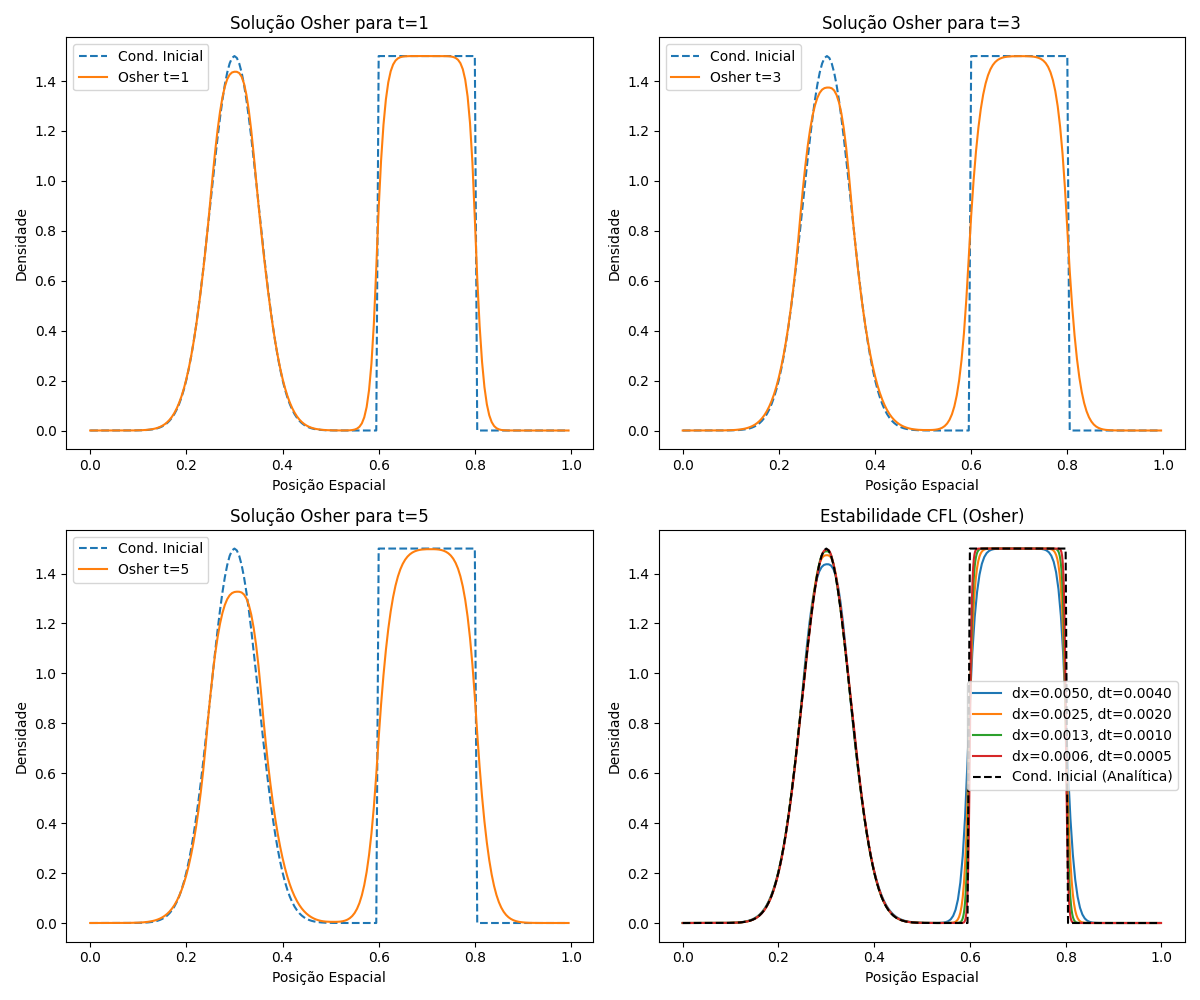
\includegraphics[width=\textwidth]{code/images/Osher.png}
    \caption{Solução Osher para $t=1$, $t=3$ e $t=5$, com a condição inicial representada pela linha tracejada.}
    \label{fig:osher}
\end{figure}

\subsection{Análise dos Resultados do Método Osher}

A Figura \ref{fig:osher} apresenta a evolução da solução obtida pelo método Osher nos tempos \(t=1\), \(t=3\) e \(t=5\), comparando a solução numérica com a condição inicial (\(t=0\)).

- \textbf{Condição inicial (\(t=0\))}: A condição inicial utilizada é uma combinação de uma função gaussiana centrada em \(x=0,3\) e uma concentração uniforme entre \(x=0,6\) e \(x=0,8\).
- \textbf{Incremento de tempo (\(\Delta t\))}: O número de Courant \(C=0,8\) foi aplicado para calcular o passo de tempo, garantindo estabilidade conforme a condição CFL.

Os gráficos mostram que o método Osher preserva de forma eficiente a monotonicidade e a forma geral do perfil de concentração ao longo do tempo, minimizando oscilações. Em \(t=1\), a solução numérica está bem próxima da condição inicial, com pequenas diferenças no topo da gaussiana e nas bordas da concentração uniforme. Para \(t=3\) e \(t=5\), o método continua apresentando um comportamento estável, preservando a forma da gaussiana e do degrau, mas com leves atenuações devido à dissipação numérica.

\begin{table}[H]
    \centering
    \begin{tabular}{rrrrrr}
\toprule
Posicao Espacial & Condicao Inicial & Osher t=1 & Osher t=3 & Osher t=5 & Posicao da Estabilidade \\
\midrule
0.000000 & 0.000000 & 0.000000 & 0.000002 & 0.000006 & 0.000000 \\
0.050000 & 0.000006 & 0.000012 & 0.000034 & 0.000053 & 0.050000 \\
0.100000 & 0.000503 & 0.000718 & 0.001223 & 0.001420 & 0.100000 \\
0.150000 & 0.016663 & 0.018961 & 0.023321 & 0.022593 & 0.150000 \\
0.200000 & 0.203003 & 0.206288 & 0.213317 & 0.192373 & 0.200000 \\
0.250000 & 0.909796 & 0.923582 & 0.967856 & 0.912867 & 0.250000 \\
0.300000 & 1.500000 & 1.437160 & 1.373804 & 1.325958 & 0.300000 \\
0.350000 & 0.909796 & 0.904268 & 0.930223 & 1.030586 & 0.350000 \\
0.400000 & 0.203003 & 0.208248 & 0.218056 & 0.261015 & 0.400000 \\
0.450000 & 0.016663 & 0.019849 & 0.025923 & 0.037466 & 0.450000 \\
0.500000 & 0.000503 & 0.000766 & 0.001917 & 0.004691 & 0.500000 \\
0.550000 & 0.000006 & 0.003678 & 0.028017 & 0.040087 & 0.550000 \\
0.600000 & 1.500000 & 0.890163 & 0.860449 & 0.740881 & 0.600000 \\
0.650000 & 1.500000 & 1.497814 & 1.475949 & 1.438465 & 0.650000 \\
0.700000 & 1.500000 & 1.500000 & 1.499627 & 1.497384 & 0.700000 \\
0.750000 & 1.500000 & 1.498258 & 1.481938 & 1.472013 & 0.750000 \\
0.800000 & 1.500000 & 0.849292 & 0.804179 & 0.905699 & 0.800000 \\
0.850000 & 0.000000 & 0.004615 & 0.036054 & 0.083578 & 0.850000 \\
0.900000 & 0.000000 & 0.000001 & 0.000308 & 0.002432 & 0.900000 \\
0.950000 & 0.000000 & 0.000000 & 0.000003 & 0.000025 & 0.950000 \\
\bottomrule
\end{tabular}

    \caption{Resultados numéricos do método Osher para posições espaciais selecionadas em $t=1$, $t=3$ e $t=5$.}
    \label{tab:osher}
\end{table}

A Tabela \ref{tab:osher} apresenta os valores numéricos da solução do método Osher em posições selecionadas do domínio para diferentes instantes de tempo. Os resultados evidenciam a precisão do método em capturar a evolução do perfil de concentração com o mínimo de oscilações ou dispersão.

\subsection{Implementação em Python}

O código em Python para o método Osher utiliza a função principal \texttt{resolverAdveccaoTVD}, que aplica o limitador e calcula a evolução da densidade ao longo do tempo. A cada passo temporal, o fluxo \(F_{i+1/2}\) é atualizado com base no limitador de Osher, garantindo estabilidade e precisão. O trecho do código é apresentado na Listagem~\ref{lst:codigo_osher}.

\begin{lstlisting}[language=Python, caption={Código para resolver a advecção usando o método Osher}, label={lst:codigo_osher}]
# Método TVD com limitador de Osher
def limitadorOsher(theta):
    return np.maximum(0, np.minimum(1, theta))

def metodoTvdOsher(densidade, nt, intervaloTempo, intervaloEspacial, numeroCourant):
    """
    Método TVD para resolver a advecção utilizando o limitador de Osher.
    """
    for n in range(nt):
        novaDensidade = densidade.copy()
        for i in range(len(densidade)):
            esquerda = (i - 1) % len(densidade)
            direita = (i + 1) % len(densidade)
            # Calcula o gradiente relativo (theta)
            theta = (densidade[i] - densidade[esquerda]) / (densidade[direita] - densidade[i] + 1e-6)
            # Fluxos para direita e esquerda
            fluxoDireita = densidade[i] + 0.5 * numeroCourant * (1 - numeroCourant) * limitadorOsher(theta) * (densidade[direita] - densidade[i])
            fluxoEsquerda = densidade[esquerda] + 0.5 * numeroCourant * (1 - numeroCourant) * limitadorOsher(theta) * (densidade[i] - densidade[esquerda])
            # Atualiza a densidade
            novaDensidade[i] = densidade[i] - numeroCourant * (fluxoDireita - fluxoEsquerda)
        densidade = novaDensidade.copy()
    return densidade
\end{lstlisting}


A implementação do método Osher utiliza o limitador \texttt{limitadorOsher} para controlar os fluxos numéricos em cada passo temporal, garantindo estabilidade e precisão. O número de Courant \(C = 0,8\) é aplicado para satisfazer a condição CFL, essencial para a convergência das soluções numéricas.
 % Completa e Validada
\subsection{O Método Osher}

O método Osher, baseado no limitador de variação total diminuída (TVD), é projetado para preservar a monotonicidade e minimizar oscilações em regiões com gradientes acentuados. Sua implementação utiliza fluxos numéricos controlados por um limitador, definido como:
\[
    \phi_{\text{lim}}(\theta) = \max(0, \min(1, \theta)),
\]
onde \(\theta\) é uma razão local dos gradientes calculados em cada ponto do domínio.

A solução numérica do método Osher é baseada na atualização iterativa da equação da advecção discretizada em um esquema de volumes finitos:
\[
    Q_i^{n+1} = Q_i^n - C (F_{i+1/2} - F_{i-1/2}),
\]
com o fluxo \(F_{i+1/2}\) controlado pelo limitador \(\phi_{\text{lim}}\).

\begin{figure}[H]
    \centering
    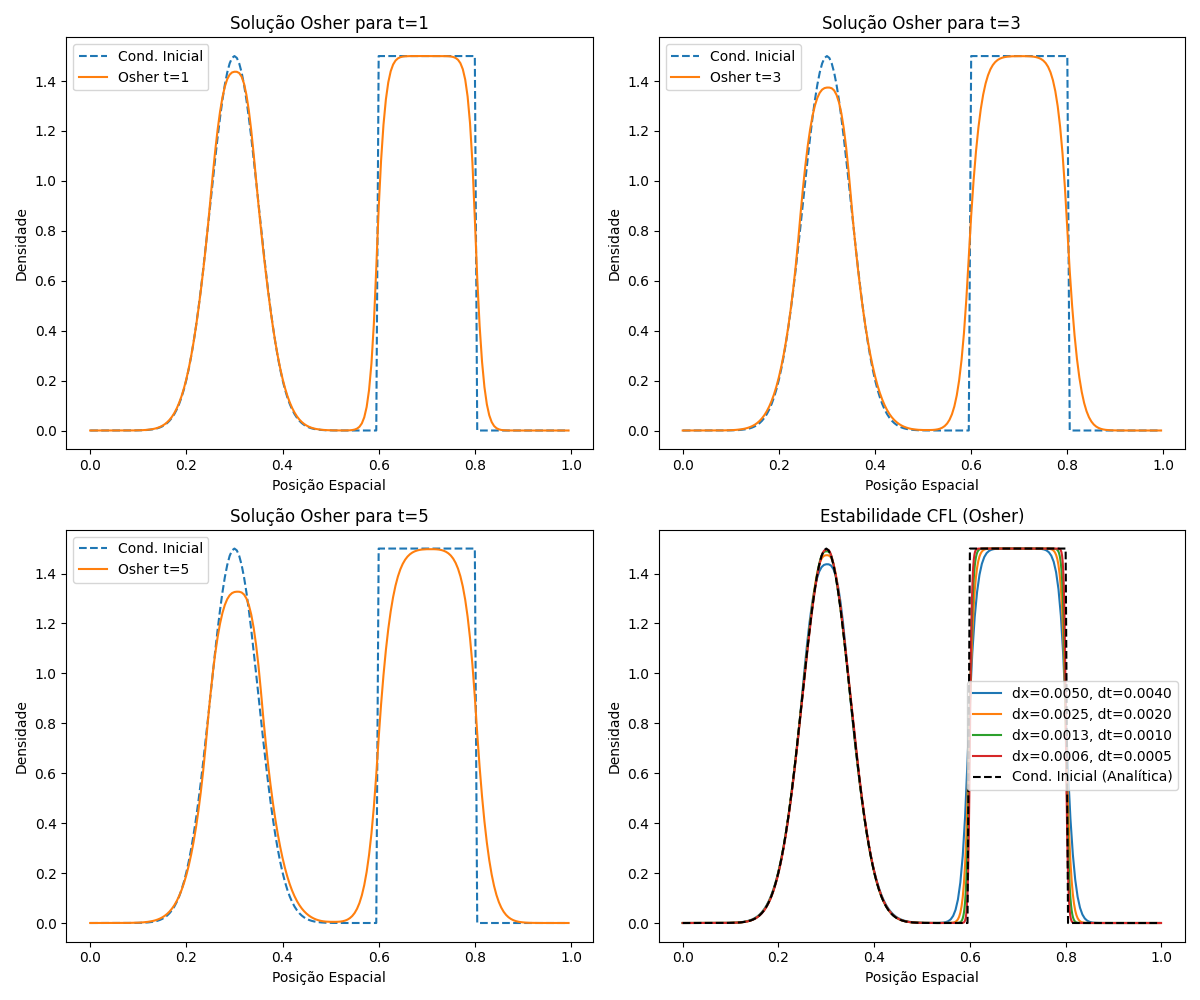
\includegraphics[width=\textwidth]{code/images/Osher.png}
    \caption{Solução Osher para $t=1$, $t=3$ e $t=5$, com a condição inicial representada pela linha tracejada.}
    \label{fig:osher}
\end{figure}

\subsection{Análise dos Resultados do Método Osher}

A Figura \ref{fig:osher} apresenta a evolução da solução obtida pelo método Osher nos tempos \(t=1\), \(t=3\) e \(t=5\), comparando a solução numérica com a condição inicial (\(t=0\)).

- \textbf{Condição inicial (\(t=0\))}: A condição inicial utilizada é uma combinação de uma função gaussiana centrada em \(x=0,3\) e uma concentração uniforme entre \(x=0,6\) e \(x=0,8\).
- \textbf{Incremento de tempo (\(\Delta t\))}: O número de Courant \(C=0,8\) foi aplicado para calcular o passo de tempo, garantindo estabilidade conforme a condição CFL.

Os gráficos mostram que o método Osher preserva de forma eficiente a monotonicidade e a forma geral do perfil de concentração ao longo do tempo, minimizando oscilações. Em \(t=1\), a solução numérica está bem próxima da condição inicial, com pequenas diferenças no topo da gaussiana e nas bordas da concentração uniforme. Para \(t=3\) e \(t=5\), o método continua apresentando um comportamento estável, preservando a forma da gaussiana e do degrau, mas com leves atenuações devido à dissipação numérica.

\begin{table}[H]
    \centering
    \begin{tabular}{rrrrrr}
\toprule
Posicao Espacial & Condicao Inicial & Osher t=1 & Osher t=3 & Osher t=5 & Posicao da Estabilidade \\
\midrule
0.000000 & 0.000000 & 0.000000 & 0.000002 & 0.000006 & 0.000000 \\
0.050000 & 0.000006 & 0.000012 & 0.000034 & 0.000053 & 0.050000 \\
0.100000 & 0.000503 & 0.000718 & 0.001223 & 0.001420 & 0.100000 \\
0.150000 & 0.016663 & 0.018961 & 0.023321 & 0.022593 & 0.150000 \\
0.200000 & 0.203003 & 0.206288 & 0.213317 & 0.192373 & 0.200000 \\
0.250000 & 0.909796 & 0.923582 & 0.967856 & 0.912867 & 0.250000 \\
0.300000 & 1.500000 & 1.437160 & 1.373804 & 1.325958 & 0.300000 \\
0.350000 & 0.909796 & 0.904268 & 0.930223 & 1.030586 & 0.350000 \\
0.400000 & 0.203003 & 0.208248 & 0.218056 & 0.261015 & 0.400000 \\
0.450000 & 0.016663 & 0.019849 & 0.025923 & 0.037466 & 0.450000 \\
0.500000 & 0.000503 & 0.000766 & 0.001917 & 0.004691 & 0.500000 \\
0.550000 & 0.000006 & 0.003678 & 0.028017 & 0.040087 & 0.550000 \\
0.600000 & 1.500000 & 0.890163 & 0.860449 & 0.740881 & 0.600000 \\
0.650000 & 1.500000 & 1.497814 & 1.475949 & 1.438465 & 0.650000 \\
0.700000 & 1.500000 & 1.500000 & 1.499627 & 1.497384 & 0.700000 \\
0.750000 & 1.500000 & 1.498258 & 1.481938 & 1.472013 & 0.750000 \\
0.800000 & 1.500000 & 0.849292 & 0.804179 & 0.905699 & 0.800000 \\
0.850000 & 0.000000 & 0.004615 & 0.036054 & 0.083578 & 0.850000 \\
0.900000 & 0.000000 & 0.000001 & 0.000308 & 0.002432 & 0.900000 \\
0.950000 & 0.000000 & 0.000000 & 0.000003 & 0.000025 & 0.950000 \\
\bottomrule
\end{tabular}

    \caption{Resultados numéricos do método Osher para posições espaciais selecionadas em $t=1$, $t=3$ e $t=5$.}
    \label{tab:osher}
\end{table}

A Tabela \ref{tab:osher} apresenta os valores numéricos da solução do método Osher em posições selecionadas do domínio para diferentes instantes de tempo. Os resultados evidenciam a precisão do método em capturar a evolução do perfil de concentração com o mínimo de oscilações ou dispersão.

\subsection{Implementação em Python}

O código em Python para o método Osher utiliza a função principal \texttt{resolverAdveccaoTVD}, que aplica o limitador e calcula a evolução da densidade ao longo do tempo. A cada passo temporal, o fluxo \(F_{i+1/2}\) é atualizado com base no limitador de Osher, garantindo estabilidade e precisão. O trecho do código é apresentado na Listagem~\ref{lst:codigo_osher}.

\begin{lstlisting}[language=Python, caption={Código para resolver a advecção usando o método Osher}, label={lst:codigo_osher}]
# Método TVD com limitador de Osher
def limitadorOsher(theta):
    return np.maximum(0, np.minimum(1, theta))

def metodoTvdOsher(densidade, nt, intervaloTempo, intervaloEspacial, numeroCourant):
    """
    Método TVD para resolver a advecção utilizando o limitador de Osher.
    """
    for n in range(nt):
        novaDensidade = densidade.copy()
        for i in range(len(densidade)):
            esquerda = (i - 1) % len(densidade)
            direita = (i + 1) % len(densidade)
            # Calcula o gradiente relativo (theta)
            theta = (densidade[i] - densidade[esquerda]) / (densidade[direita] - densidade[i] + 1e-6)
            # Fluxos para direita e esquerda
            fluxoDireita = densidade[i] + 0.5 * numeroCourant * (1 - numeroCourant) * limitadorOsher(theta) * (densidade[direita] - densidade[i])
            fluxoEsquerda = densidade[esquerda] + 0.5 * numeroCourant * (1 - numeroCourant) * limitadorOsher(theta) * (densidade[i] - densidade[esquerda])
            # Atualiza a densidade
            novaDensidade[i] = densidade[i] - numeroCourant * (fluxoDireita - fluxoEsquerda)
        densidade = novaDensidade.copy()
    return densidade
\end{lstlisting}


A implementação do método Osher utiliza o limitador \texttt{limitadorOsher} para controlar os fluxos numéricos em cada passo temporal, garantindo estabilidade e precisão. O número de Courant \(C = 0,8\) é aplicado para satisfazer a condição CFL, essencial para a convergência das soluções numéricas.
 % Completa e Validada
\subsection{O Método Osher}

O método Osher, baseado no limitador de variação total diminuída (TVD), é projetado para preservar a monotonicidade e minimizar oscilações em regiões com gradientes acentuados. Sua implementação utiliza fluxos numéricos controlados por um limitador, definido como:
\[
    \phi_{\text{lim}}(\theta) = \max(0, \min(1, \theta)),
\]
onde \(\theta\) é uma razão local dos gradientes calculados em cada ponto do domínio.

A solução numérica do método Osher é baseada na atualização iterativa da equação da advecção discretizada em um esquema de volumes finitos:
\[
    Q_i^{n+1} = Q_i^n - C (F_{i+1/2} - F_{i-1/2}),
\]
com o fluxo \(F_{i+1/2}\) controlado pelo limitador \(\phi_{\text{lim}}\).

\begin{figure}[H]
    \centering
    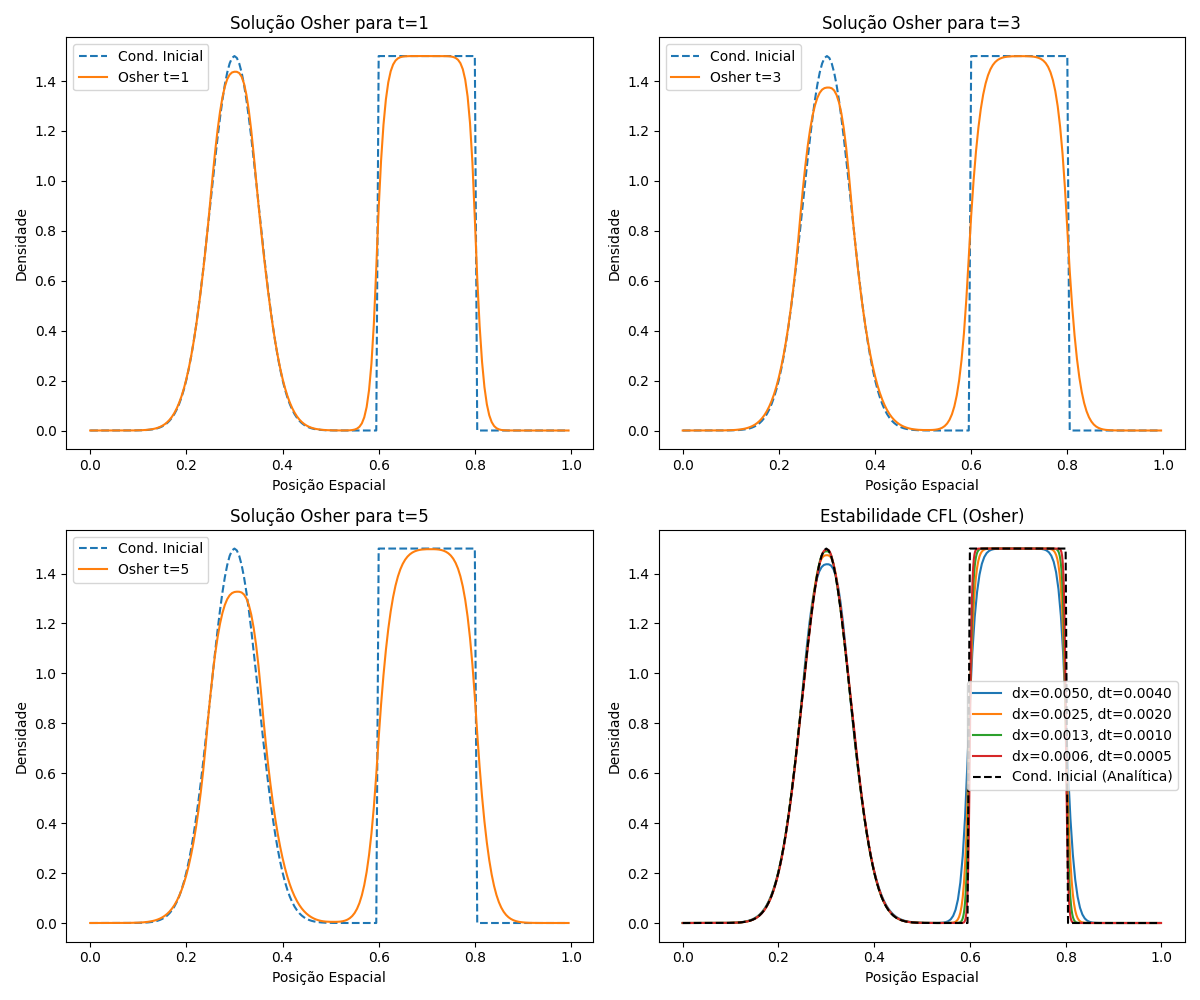
\includegraphics[width=\textwidth]{code/images/Osher.png}
    \caption{Solução Osher para $t=1$, $t=3$ e $t=5$, com a condição inicial representada pela linha tracejada.}
    \label{fig:osher}
\end{figure}

\subsection{Análise dos Resultados do Método Osher}

A Figura \ref{fig:osher} apresenta a evolução da solução obtida pelo método Osher nos tempos \(t=1\), \(t=3\) e \(t=5\), comparando a solução numérica com a condição inicial (\(t=0\)).

- \textbf{Condição inicial (\(t=0\))}: A condição inicial utilizada é uma combinação de uma função gaussiana centrada em \(x=0,3\) e uma concentração uniforme entre \(x=0,6\) e \(x=0,8\).
- \textbf{Incremento de tempo (\(\Delta t\))}: O número de Courant \(C=0,8\) foi aplicado para calcular o passo de tempo, garantindo estabilidade conforme a condição CFL.

Os gráficos mostram que o método Osher preserva de forma eficiente a monotonicidade e a forma geral do perfil de concentração ao longo do tempo, minimizando oscilações. Em \(t=1\), a solução numérica está bem próxima da condição inicial, com pequenas diferenças no topo da gaussiana e nas bordas da concentração uniforme. Para \(t=3\) e \(t=5\), o método continua apresentando um comportamento estável, preservando a forma da gaussiana e do degrau, mas com leves atenuações devido à dissipação numérica.

\begin{table}[H]
    \centering
    \begin{tabular}{rrrrrr}
\toprule
Posicao Espacial & Condicao Inicial & Osher t=1 & Osher t=3 & Osher t=5 & Posicao da Estabilidade \\
\midrule
0.000000 & 0.000000 & 0.000000 & 0.000002 & 0.000006 & 0.000000 \\
0.050000 & 0.000006 & 0.000012 & 0.000034 & 0.000053 & 0.050000 \\
0.100000 & 0.000503 & 0.000718 & 0.001223 & 0.001420 & 0.100000 \\
0.150000 & 0.016663 & 0.018961 & 0.023321 & 0.022593 & 0.150000 \\
0.200000 & 0.203003 & 0.206288 & 0.213317 & 0.192373 & 0.200000 \\
0.250000 & 0.909796 & 0.923582 & 0.967856 & 0.912867 & 0.250000 \\
0.300000 & 1.500000 & 1.437160 & 1.373804 & 1.325958 & 0.300000 \\
0.350000 & 0.909796 & 0.904268 & 0.930223 & 1.030586 & 0.350000 \\
0.400000 & 0.203003 & 0.208248 & 0.218056 & 0.261015 & 0.400000 \\
0.450000 & 0.016663 & 0.019849 & 0.025923 & 0.037466 & 0.450000 \\
0.500000 & 0.000503 & 0.000766 & 0.001917 & 0.004691 & 0.500000 \\
0.550000 & 0.000006 & 0.003678 & 0.028017 & 0.040087 & 0.550000 \\
0.600000 & 1.500000 & 0.890163 & 0.860449 & 0.740881 & 0.600000 \\
0.650000 & 1.500000 & 1.497814 & 1.475949 & 1.438465 & 0.650000 \\
0.700000 & 1.500000 & 1.500000 & 1.499627 & 1.497384 & 0.700000 \\
0.750000 & 1.500000 & 1.498258 & 1.481938 & 1.472013 & 0.750000 \\
0.800000 & 1.500000 & 0.849292 & 0.804179 & 0.905699 & 0.800000 \\
0.850000 & 0.000000 & 0.004615 & 0.036054 & 0.083578 & 0.850000 \\
0.900000 & 0.000000 & 0.000001 & 0.000308 & 0.002432 & 0.900000 \\
0.950000 & 0.000000 & 0.000000 & 0.000003 & 0.000025 & 0.950000 \\
\bottomrule
\end{tabular}

    \caption{Resultados numéricos do método Osher para posições espaciais selecionadas em $t=1$, $t=3$ e $t=5$.}
    \label{tab:osher}
\end{table}

A Tabela \ref{tab:osher} apresenta os valores numéricos da solução do método Osher em posições selecionadas do domínio para diferentes instantes de tempo. Os resultados evidenciam a precisão do método em capturar a evolução do perfil de concentração com o mínimo de oscilações ou dispersão.

\subsection{Implementação em Python}

O código em Python para o método Osher utiliza a função principal \texttt{resolverAdveccaoTVD}, que aplica o limitador e calcula a evolução da densidade ao longo do tempo. A cada passo temporal, o fluxo \(F_{i+1/2}\) é atualizado com base no limitador de Osher, garantindo estabilidade e precisão. O trecho do código é apresentado na Listagem~\ref{lst:codigo_osher}.

\begin{lstlisting}[language=Python, caption={Código para resolver a advecção usando o método Osher}, label={lst:codigo_osher}]
# Método TVD com limitador de Osher
def limitadorOsher(theta):
    return np.maximum(0, np.minimum(1, theta))

def metodoTvdOsher(densidade, nt, intervaloTempo, intervaloEspacial, numeroCourant):
    """
    Método TVD para resolver a advecção utilizando o limitador de Osher.
    """
    for n in range(nt):
        novaDensidade = densidade.copy()
        for i in range(len(densidade)):
            esquerda = (i - 1) % len(densidade)
            direita = (i + 1) % len(densidade)
            # Calcula o gradiente relativo (theta)
            theta = (densidade[i] - densidade[esquerda]) / (densidade[direita] - densidade[i] + 1e-6)
            # Fluxos para direita e esquerda
            fluxoDireita = densidade[i] + 0.5 * numeroCourant * (1 - numeroCourant) * limitadorOsher(theta) * (densidade[direita] - densidade[i])
            fluxoEsquerda = densidade[esquerda] + 0.5 * numeroCourant * (1 - numeroCourant) * limitadorOsher(theta) * (densidade[i] - densidade[esquerda])
            # Atualiza a densidade
            novaDensidade[i] = densidade[i] - numeroCourant * (fluxoDireita - fluxoEsquerda)
        densidade = novaDensidade.copy()
    return densidade
\end{lstlisting}


A implementação do método Osher utiliza o limitador \texttt{limitadorOsher} para controlar os fluxos numéricos em cada passo temporal, garantindo estabilidade e precisão. O número de Courant \(C = 0,8\) é aplicado para satisfazer a condição CFL, essencial para a convergência das soluções numéricas.
 % Completa e Validada

% ===============================================================
% Conclusão geral ===============================================
\section{Desenvolvimento Teórico}

A equação de advecção unidimensional descreve o transporte de uma quantidade conservada, como a concentração de um traçador, ao longo de um eixo espacial. Para resolver essa equação numericamente, é utilizado o método dos Volumes Finitos, que permite a discretização do espaço e do tempo, garantindo uma formulação adequada para a conservação da quantidade transportada \cite{leveque2002finite}. A equação de advecção, em sua forma conservativa, é dada por:

\begin{equation}
    \frac{\partial \Phi}{\partial t} + \frac{\partial}{\partial x} (u \Phi) = 0,
\end{equation}

onde $\Phi$ representa a variável dependente (concentração do traçador) e $u$ é a velocidade de advecção. Com $u$ constante, a equação simplifica-se para:

\begin{equation}
    \frac{\partial \Phi}{\partial t} + u \frac{\partial \Phi}{\partial x} = 0.
\end{equation}

Neste trabalho, a solução numérica é obtida utilizando métodos do tipo \textbf{TVD (Total Variation Diminishing)}. Esses métodos são amplamente reconhecidos por sua capacidade de preservar a monotonicidade da solução e evitar oscilações artificiais, especialmente em regiões com gradientes acentuados ou descontinuidades \cite{harten1983high}. Os métodos implementados são:

\begin{itemize}
    \item \textbf{Limitador de Osher}: Este limitador é projetado para reduzir oscilações artificiais e garantir que a solução permaneça monotônica. Ele é definido como:
          \[
              \phi_{\text{lim}}(\theta) = \max(0, \min(1, \theta)),
          \]
          onde $\theta$ é uma medida da variação local da solução \cite{osher1984rktvd}.

    \item \textbf{Limitador de Sweby}: Este limitador permite maior controle sobre a dissipação, introduzindo um parâmetro ajustável $\beta$. Sua formulação é:
          \[
              \phi_{\text{lim}}(\theta) = \max(0, \min(\beta \theta, \min(1, \theta))),
          \]
          onde valores típicos de $\beta$ estão na faixa $1 \leq \beta \leq 2$ \cite{sweby1984high}.

    \item \textbf{Limitador de Van Albada}: Este limitador equilibra suavidade e precisão, sendo especialmente útil em regiões de gradientes suaves. Sua definição é:
          \[
              \phi_{\text{lim}}(\theta) = \frac{\theta + \theta^2}{1 + \theta^2}.
          \]
          Este limitador é amplamente utilizado devido à sua estabilidade em problemas com gradientes suaves \cite{vanalbada1982family}.
\end{itemize}

Para garantir a estabilidade das simulações, o número de Courant é fixado em $C = 0,8$, respeitando a condição CFL \cite{leveque2002finite}. A condição inicial é definida por uma função composta de uma gaussiana e um valor constante em um intervalo específico, representando um perfil inicial com gradientes suaves e regiões de concentração uniforme. As simulações são realizadas para os instantes de tempo $t = 1$ e $t = 5$, sob condições de contorno periódicas.

Os fluxos nas interfaces dos volumes finitos são calculados considerando os termos anti-difusivos controlados pelos limitadores. A formulação geral do fluxo numérico nos métodos TVD é dada por:
\[
    F_{i+1/2} = u \Phi_i + \frac{u}{2}(1 - C) \phi_{\text{lim}}(\theta_i)(\Phi_{i+1} - \Phi_i),
\]
onde $\theta_i$ é a razão entre os gradientes locais definidos para o intervalo \cite{leveque2002finite}.

Os resultados obtidos serão analisados com gráficos que comparam a solução analítica com as soluções numéricas, permitindo observar a influência de cada limitador na dissipação e dispersão do perfil inicial. Além disso, tabelas apresentarão valores em pontos específicos do domínio para uma análise quantitativa da precisão de cada método.


% ===============================================================
% Referencias ===================================================
\section{Desenvolvimento Teórico}

A equação de advecção unidimensional descreve o transporte de uma quantidade conservada, como a concentração de um traçador, ao longo de um eixo espacial. Para resolver essa equação numericamente, é utilizado o método dos Volumes Finitos, que permite a discretização do espaço e do tempo, garantindo uma formulação adequada para a conservação da quantidade transportada \cite{leveque2002finite}. A equação de advecção, em sua forma conservativa, é dada por:

\begin{equation}
    \frac{\partial \Phi}{\partial t} + \frac{\partial}{\partial x} (u \Phi) = 0,
\end{equation}

onde $\Phi$ representa a variável dependente (concentração do traçador) e $u$ é a velocidade de advecção. Com $u$ constante, a equação simplifica-se para:

\begin{equation}
    \frac{\partial \Phi}{\partial t} + u \frac{\partial \Phi}{\partial x} = 0.
\end{equation}

Neste trabalho, a solução numérica é obtida utilizando métodos do tipo \textbf{TVD (Total Variation Diminishing)}. Esses métodos são amplamente reconhecidos por sua capacidade de preservar a monotonicidade da solução e evitar oscilações artificiais, especialmente em regiões com gradientes acentuados ou descontinuidades \cite{harten1983high}. Os métodos implementados são:

\begin{itemize}
    \item \textbf{Limitador de Osher}: Este limitador é projetado para reduzir oscilações artificiais e garantir que a solução permaneça monotônica. Ele é definido como:
          \[
              \phi_{\text{lim}}(\theta) = \max(0, \min(1, \theta)),
          \]
          onde $\theta$ é uma medida da variação local da solução \cite{osher1984rktvd}.

    \item \textbf{Limitador de Sweby}: Este limitador permite maior controle sobre a dissipação, introduzindo um parâmetro ajustável $\beta$. Sua formulação é:
          \[
              \phi_{\text{lim}}(\theta) = \max(0, \min(\beta \theta, \min(1, \theta))),
          \]
          onde valores típicos de $\beta$ estão na faixa $1 \leq \beta \leq 2$ \cite{sweby1984high}.

    \item \textbf{Limitador de Van Albada}: Este limitador equilibra suavidade e precisão, sendo especialmente útil em regiões de gradientes suaves. Sua definição é:
          \[
              \phi_{\text{lim}}(\theta) = \frac{\theta + \theta^2}{1 + \theta^2}.
          \]
          Este limitador é amplamente utilizado devido à sua estabilidade em problemas com gradientes suaves \cite{vanalbada1982family}.
\end{itemize}

Para garantir a estabilidade das simulações, o número de Courant é fixado em $C = 0,8$, respeitando a condição CFL \cite{leveque2002finite}. A condição inicial é definida por uma função composta de uma gaussiana e um valor constante em um intervalo específico, representando um perfil inicial com gradientes suaves e regiões de concentração uniforme. As simulações são realizadas para os instantes de tempo $t = 1$ e $t = 5$, sob condições de contorno periódicas.

Os fluxos nas interfaces dos volumes finitos são calculados considerando os termos anti-difusivos controlados pelos limitadores. A formulação geral do fluxo numérico nos métodos TVD é dada por:
\[
    F_{i+1/2} = u \Phi_i + \frac{u}{2}(1 - C) \phi_{\text{lim}}(\theta_i)(\Phi_{i+1} - \Phi_i),
\]
onde $\theta_i$ é a razão entre os gradientes locais definidos para o intervalo \cite{leveque2002finite}.

Os resultados obtidos serão analisados com gráficos que comparam a solução analítica com as soluções numéricas, permitindo observar a influência de cada limitador na dissipação e dispersão do perfil inicial. Além disso, tabelas apresentarão valores em pontos específicos do domínio para uma análise quantitativa da precisão de cada método.


% ===============================================================
% Anexo ou Apendices ============================================
\section{Desenvolvimento Teórico}

A equação de advecção unidimensional descreve o transporte de uma quantidade conservada, como a concentração de um traçador, ao longo de um eixo espacial. Para resolver essa equação numericamente, é utilizado o método dos Volumes Finitos, que permite a discretização do espaço e do tempo, garantindo uma formulação adequada para a conservação da quantidade transportada \cite{leveque2002finite}. A equação de advecção, em sua forma conservativa, é dada por:

\begin{equation}
    \frac{\partial \Phi}{\partial t} + \frac{\partial}{\partial x} (u \Phi) = 0,
\end{equation}

onde $\Phi$ representa a variável dependente (concentração do traçador) e $u$ é a velocidade de advecção. Com $u$ constante, a equação simplifica-se para:

\begin{equation}
    \frac{\partial \Phi}{\partial t} + u \frac{\partial \Phi}{\partial x} = 0.
\end{equation}

Neste trabalho, a solução numérica é obtida utilizando métodos do tipo \textbf{TVD (Total Variation Diminishing)}. Esses métodos são amplamente reconhecidos por sua capacidade de preservar a monotonicidade da solução e evitar oscilações artificiais, especialmente em regiões com gradientes acentuados ou descontinuidades \cite{harten1983high}. Os métodos implementados são:

\begin{itemize}
    \item \textbf{Limitador de Osher}: Este limitador é projetado para reduzir oscilações artificiais e garantir que a solução permaneça monotônica. Ele é definido como:
          \[
              \phi_{\text{lim}}(\theta) = \max(0, \min(1, \theta)),
          \]
          onde $\theta$ é uma medida da variação local da solução \cite{osher1984rktvd}.

    \item \textbf{Limitador de Sweby}: Este limitador permite maior controle sobre a dissipação, introduzindo um parâmetro ajustável $\beta$. Sua formulação é:
          \[
              \phi_{\text{lim}}(\theta) = \max(0, \min(\beta \theta, \min(1, \theta))),
          \]
          onde valores típicos de $\beta$ estão na faixa $1 \leq \beta \leq 2$ \cite{sweby1984high}.

    \item \textbf{Limitador de Van Albada}: Este limitador equilibra suavidade e precisão, sendo especialmente útil em regiões de gradientes suaves. Sua definição é:
          \[
              \phi_{\text{lim}}(\theta) = \frac{\theta + \theta^2}{1 + \theta^2}.
          \]
          Este limitador é amplamente utilizado devido à sua estabilidade em problemas com gradientes suaves \cite{vanalbada1982family}.
\end{itemize}

Para garantir a estabilidade das simulações, o número de Courant é fixado em $C = 0,8$, respeitando a condição CFL \cite{leveque2002finite}. A condição inicial é definida por uma função composta de uma gaussiana e um valor constante em um intervalo específico, representando um perfil inicial com gradientes suaves e regiões de concentração uniforme. As simulações são realizadas para os instantes de tempo $t = 1$ e $t = 5$, sob condições de contorno periódicas.

Os fluxos nas interfaces dos volumes finitos são calculados considerando os termos anti-difusivos controlados pelos limitadores. A formulação geral do fluxo numérico nos métodos TVD é dada por:
\[
    F_{i+1/2} = u \Phi_i + \frac{u}{2}(1 - C) \phi_{\text{lim}}(\theta_i)(\Phi_{i+1} - \Phi_i),
\]
onde $\theta_i$ é a razão entre os gradientes locais definidos para o intervalo \cite{leveque2002finite}.

Os resultados obtidos serão analisados com gráficos que comparam a solução analítica com as soluções numéricas, permitindo observar a influência de cada limitador na dissipação e dispersão do perfil inicial. Além disso, tabelas apresentarão valores em pontos específicos do domínio para uma análise quantitativa da precisão de cada método.


% ===============================================================
% End Document ==================================================
\end{document}

